\documentclass[../main.tex]{subfiles}

\begin{document}
	\section{Adjusting Accounts and Preparing Financial Statements}
	
	To provide timely information, accounting systems prepare reports at 
	regular intervals. This results in an accounting process impacted by the 
	time period (or periodicity) assumption. The \textbf{time period 
	assumption} 
	presumes that an organization’s activities can be divided into specific 
	time periods such as a month, a three-month quarter, a six-month interval, 
	or a year. Most organizations use a year as their primary accounting 
	period. Many organizations also prepare interim financial statements 
	covering one, three, or six months of activity.
	
	\begin{figure}[ht]
		\centering
		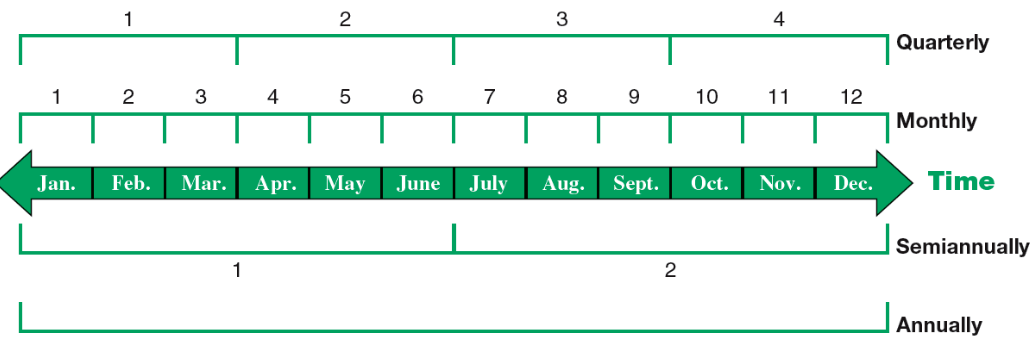
\includegraphics[width=1\columnwidth]{images/c3/accounting_period.png}
	\end{figure}
	
	When we divide business activities into arbitrary fixed periods of time, it 
	is often necessary to have special accounting for transactions that cross 
	from one time period to the next.
	
	\subsection{Accrual Basis vs. Cash Basis}
	
	The \textbf{accrual basis} dictates that revenues be recognized when earned 
	and expenses be recognized when incurred. The accrual basis of accounting 
	is considered to be in compliance with generally accepted accounting 
	principles, or GAAP.
	
	The \textbf{cash basis} of accounting dictates that revenues be recognized 
	when the 
	cash is actually received and that expenses are recorded when the cash is 
	paid. The cash basis is not considered to be compliant with GAAP. Almost 
	all companies follow the accrual basis of accounting. 
	
	\subsection{Accrual Basis Accounting}
	
	Accrual basis accounting, produces a better measure of the profits arising 
	from the company’s activities. According to GAAP and IFRS, the accrual 
	basis is the only acceptable method for external reporting of income. The 
	cash basis can be used internally by some small companies, but GAAP and 
	IFRS do not allow it for external reporting.
	
	The “rule of accrual” is that the financial effects of business activities 
	are measured and reported when the activities actually occur, not when the 
	cash related to them is received or paid. That is, revenues are recognized 
	when they are earned and expenses when they are incurred. The two basic 
	accounting principles that determine when revenues and expenses are 
	recognized under accrual basis accounting are called the \textbf{revenue 
	recognition} and \textbf{expense recognition principles}.

	\subsubsection{Revenue Recognition Principle}
	
	The revenue recognition principle recognizes revenue when they are earned. 
	
	All companies expect to receive cash in exchange for providing goods and 
	services, but the timing of cash receipts does not dictate when revenues 
	are recognized. Instead, the key factor in determining when to recognize 
	revenue is whether the company has provided goods or services to customers 
	during the accounting period. There are three cases:
	
	\begin{itemize}[noitemsep]
		\item The cash is received before the sale or service \eg airlines, 
		magazine publishers, insurance companies, and retail stores routinely 
		receive cash before delivering goods or services. This obligation is a 
		liability called \textbf{Unearned Revenue}, and it is recorded on the 
		balance sheet equal in amount to the cash received. Revenue 
		will be reported later, when goods or services are provided in 
		exchange.
		\item The cash is received with the sale or service. Cash and revenue 
		are reported at the same time.
		\item The cash is received after the sale or service. This situation 
		typically arises when a company sells on account. Selling on account 
		means that the company provides goods or services to a customer not for 
		cash, but instead for the right to collect cash in the future. This 
		right is an asset called \textbf{Accounts Receivable}. 
		
		When payment is received, Cash account will increase
		and Accounts Receivable account will decrease. No additional revenue is 
		reported when the payment is received because the revenue was already 
		recorded when the goods/service was delivered. 
	\end{itemize}

	\subsubsection{Expenses Recognition Principle}
	
	The expenses recognition principle records expenses in the same period as 
	the revenues with which they can be reasonably be associated with. 
	
	Under accrual basis accounting, expenses are recognized in the same period 
	as the revenues to which they relate, not necessarily the period in which 
	cash is paid for them. It is the timing of the underlying business 
	activities, not the cash payments, that dictates when expenses are 
	recognized. Three possible cases exist as to when the cash can be paid in 
	comparison to when the expense is recorded:
	\begin{itemize}[noitemsep]
		\item Cash is paid before the expense is incurred. It is common for 
		businesses to pay for something that provides benefits only in future 
		periods \eg buy office supplies now but not use them until next month. 
		Under the expense recognition principle, the expense from using these 
		supplies (Supplies Expense) is reported next month, when the supplies 
		are used to earn revenue, not in the current month, when the supplies 
		were purchased. This month, the supplies represent an asset \ie 
		Supplies.
		\item Cash is paid when the expense is incurred.
		\item Cash is paid after the expense is incurred. Most businesses 
		acquire goods or services on credit, so it is common for them to incur 
		the expense of using up the benefits of goods or services in the 
		current month, before paying for them in a later month. Because the 
		cost has not yet been paid, the balance sheet 
		reports a corresponding liability called \textbf{Accounts Payable}.
	\end{itemize}

	\subsection{Adjusting Accounts}
	
	Accounting systems are designed to record most recurring daily 
	transactions, particularly any involving cash. As cash is received or paid, 
	it is recorded in the accounting system. This focus on cash works well, 
	especially when cash receipts and payments occur in the same period as the 
	activities that lead to revenues and expenses. However, as we learned, cash 
	is not always received in the period in which the company earns the related 
	revenue; likewise, cash is not always paid in the period in which the 
	company incurs the related expense.
	
	In these situations, adjustments are made to the accounting records at the 
	end of the period to ensure assets and liabilities are reported at 
	appropriate amounts. These adjustments also ensure the related revenues and 
	expenses are reported in the proper period, as required by the revenue 
	recognition and expense recognition principles.
	
	Adjustments involve both income statement and balance sheet accounts:
	\begin{itemize}[noitemsep]
		\item In Income statements, revenues are recorded when earned. Expenses 
		are recorded in the same period as the revenues to which they relate. 
		\item In Balance Sheets, assets are reported at amounts representing 
		the economic benefits that remain at the end of the period. Liabilities 
		are reported  at amounts owed at the end of the period. 
	\end{itemize}	
	In general, adjustments can be grouped into two categories: (1) 
	\textbf{deferrals}, and (2) \textbf{accruals}.
	
	Adjustments are necessary for transactions and events that extend over more 
	than one period. It is helpful to group adjustments by the timing of cash 
	receipts or cash payments in relation to the recognition of the related 
	revenues or expenses. An adjusting entry is meant to bring an asset or 
	liability account balance to its proper amount.  
	
	\begin{figure}[ht!]
		\centering
		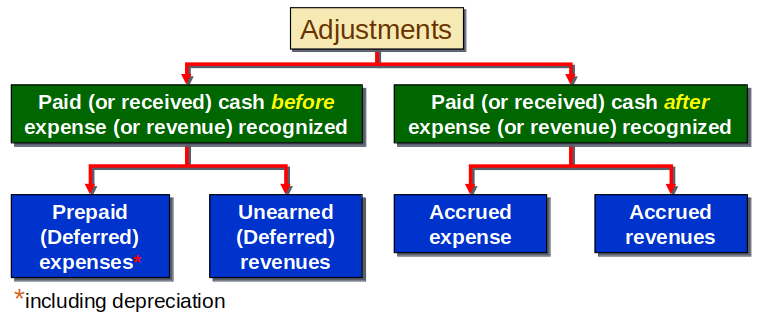
\includegraphics[width=1\columnwidth]{images/c3/framework_for_adjustments.png}
		\caption{Framework for Adjustments}	
	\end{figure}
	
	There are two broad categories of adjustments. The first is when we pay or 
	receive cash before the expense or revenue is recognized. This category 
	includes prepaid or deferred expenses (including depreciation) and unearned 
	or deferred revenues.
	
	The second major category of adjustments is when cash is paid or received 
	after the expense or revenue is recognized. This category includes accrued 
	expenses and accrued revenues.
	
	\subsubsection{Deferral Adjustments}
	
	An expense or revenue has been deferred if we have postponed reporting it 
	on the income statement until a later period. There are two key ideas in 
	deferral adjustments.
	
 	\begin{itemize}[noitemsep]
		\item Deferral adjustments are used to decrease balance sheet accounts 
		and increase corresponding income statement accounts. Previously 
		deferred amounts exist on the balance sheet because the company paid 
		cash before incurring the expense or received cash before earning 
		revenue. When revenues are earned \ie revenue 
		recognition principle or expenses incurred \ie expense 
		recognition “matching” principle, the previously deferred amounts are 
		transferred to the income statement using a deferral adjustment.
		\item Each deferral adjustment involves one asset and one expense 
		account, or one liability and one revenue account. 
	\end{itemize}
	
	\paragraph{Prepaid Expenses.}For deferred expenses, the 
	deferral adjustment is done by reducing the prepaid expense account \eg 
	Prepaid Rent and increase the expense account \eg Rent Expense at the end 
	of the period. For all adjustments involving \textbf{prepaid expenses}, we 
	increase, or debit, an expense account and reduce, or credit, an asset 
	account.
	
	\begin{figure}[ht!]
		\centering
		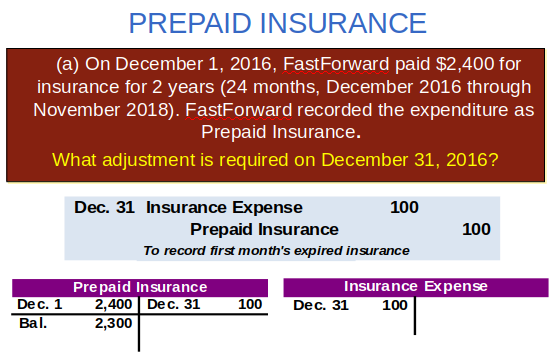
\includegraphics[width=1\columnwidth]{images/c3/prepaid_insurance_eg.png}
		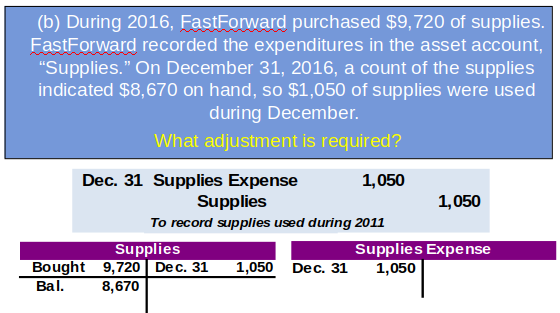
\includegraphics[width=1\columnwidth]{images/c3/supplies_eg.png}
		\caption{Prepaid Expenses Example}	
	\end{figure}
	
	Other prepaid expenses, such as Prepaid Rent, are accounted for exactly as 
	Insurance and Supplies. We should note that some prepaid expenses are both 
	paid for and fully used up within a single period. 
	
	For example, a company 
	may pay monthly rent on the first day of each month. This payment creates a 
	prepaid expense on the first day of the month that fully expires by the end 
	of the month. In these special cases, we can record the cash paid with a 
	debit to the expense account instead of an asset account.
	
	\textbf{Depreciation} is the process of allocating the cost of a piece of 
	Plant, Property and Equipment (PPE) over 
	its useful life in a systematic and rational manner.
	
	Straight-line depreciation is the most popular method used by companies. 
	They determine the amount of annual depreciation by taking the cost of the 
	plant assets, subtracting the estimated residual value, and dividing that 
	amount by the useful life of the asset. 
	\[
	\text{Depreciation Expense} = \frac{\text{Asset Cost} - \text{Residual 
	value}}{\text{Useful Life}}
	\]
	
	The residual value is the amount we 
	expect to receive for the asset when we dispose of it at the end of its 
	useful life.
	
	\begin{figure}[ht!]
		\centering
		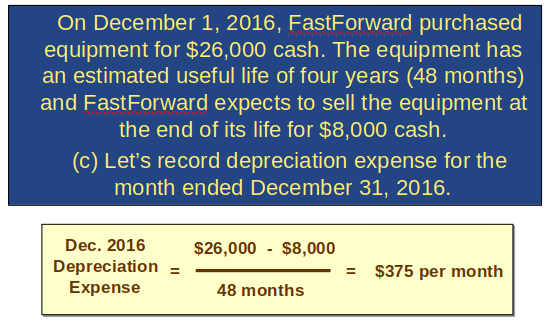
\includegraphics[width=0.8\columnwidth]{images/c3/depreciation_eg.png}
		\caption{Depreciation Example}	
	\end{figure}
	
	There are four aspects of depreciation that should be noted: 
	
	\begin{itemize}[noitemsep]
		\item \textbf{Accumulated Depreciation} is a balance sheet account and 
		\textbf{Depreciation Expense} is an income statement account. As a 
		balance sheet 
		account, Accumulated Depreciation will increase over time as it 
		accumulates the depreciation of each period until the asset is fully 
		depreciated. As an income statement account, Depreciation Expense will 
		include only the depreciation of the current accounting year.
		\item By recording depreciation in Accumulated Depreciation, distinct 
		from the Equipment account, you can report both the original cost of 
		equipment and a running total of the amount that has been depreciated. 
		This gives financial statement users a rough idea of how much of the 
		asset’s original cost (representing it’s original usefulness) has been 
		used up as of the balance sheet date.
		\item The normal balance in a \textbf{contra-account} is always the 
		opposite 
		of the account it offsets. For example, the increase in Accumulated 
		Depreciation was recorded with a credit because the account that it 
		offsets, Equipment, was previously recorded with a debit.
		\item The amount of depreciation depends on the method used for 
		determining it.	
	\end{itemize}
	
	\begin{figure}[ht!]
		\centering
		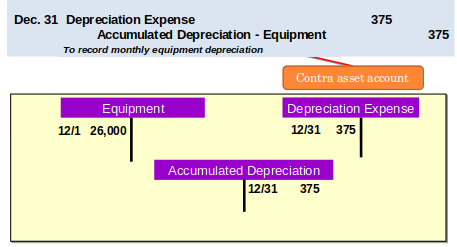
\includegraphics[width=1\columnwidth]{images/c3/recording_depreciation.png}
		\caption{\textbf{Recording Depreciation in Income Statement.} The 
		contra asset account is 
		subtracted from the related asset account. In this case, we will 
		subtract accumulated depreciation from the equipment account and report 
		the net amount on the statement of financial position.}	
	\end{figure}
	
	Cost of a piece of PPE less accumulated depreciation is known as carrying 
	amount or net book value.
	
	\begin{figure}[ht]
	\centering
	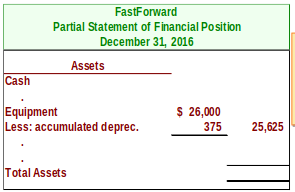
\includegraphics[width=0.8\columnwidth]{images/c3/recording_depreciation_fp.png}
		\caption{\textbf{Recording Depreciation in Balance Sheet.} Because 
		the contra account appears on the statement of financial position it 
		will not be closed at the end of the period. It will be carried forward 
		to 2017 and used to accumulate the depreciation related to the 
		equipment.}	
	\end{figure}
	
	\paragraph{Unearned Revenues.} For deferred revenues, the revenue is 
	initially deferred 
	as a liability on 
	the Balance Sheet \ie Unearned Revenue. This liability indicates the 
	company's obligation to provide a service/product in the future. Later, 
	when the company fulfills its obligation, a deferral adjustment is made to 
	reduce Unearned Revenue on the balance sheet and increase revenue account 
	\eg Sales Revenue on the income statement.
	
	When accounting for deferred revenues, we are faced with a transaction 
	where cash is received in advance of providing a product or service. In 
	this case, we prepare an adjustment for deferred revenues (a liability).  
	We always debit, or reduce, a liability account and credit, or increase, a 
	revenue account during adjustments.
	
 	\begin{figure}[ht]
	 	\centering
	 	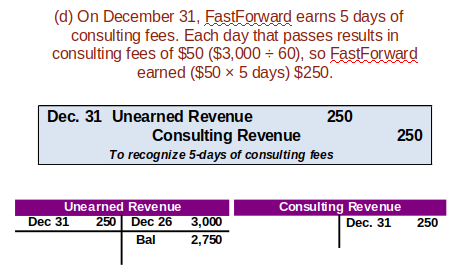
\includegraphics[width=0.9\columnwidth]{images/c3/unearned_revenue_income.png}
	 	\caption{Recording Unearned Revenue in Income Statement}	
	 \end{figure}
	
	\subsubsection{Accrual Adjustments}
	
	Accrual adjustments are needed when a company has earned revenue or 
	incurred an expense in the current period but has not yet recorded it 
	because the related cash will not be received or paid until a later period.
	
	There are two key ideas to note in accrual adjustments:
	\begin{itemize}[noitemsep]
		\item Accrual adjustments are used to record revenue or expenses when 
		they occur prior to receiving or paying cash, and to adjust 
		corresponding balance sheet accounts.
		\item Each accrual adjustment involves one asset and one revenue 
		account, or one liability and one expense account.
	\end{itemize}
	
	\paragraph{Accrued Expenses}
	
	An accrued expense is a liability relating to an expense incurred in the 
	current period that is both unpaid and unrecorded \eg credit card.
	
 	\begin{figure}[ht!]
		\centering
		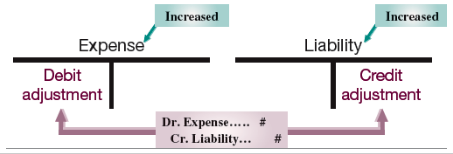
\includegraphics[width=0.8\columnwidth]{images/c3/accured_expenses.png}
		\caption{Accrued Expenses}	
	\end{figure}
	
	For all accrued expense adjusting entries, we debit, or increase an expense 
	account, and credit, or increase, a liability account.
	
 	\begin{figure}[ht!]
		\centering
		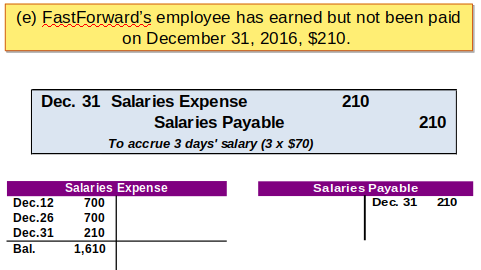
\includegraphics[width=0.9\columnwidth]{images/c3/accured_expense_eg1.png}
		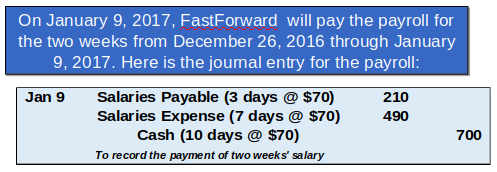
\includegraphics[width=0.9\columnwidth]{images/c3/accured_expense_eg2.png}
		\caption{Accrued Expense Example}	
	\end{figure}
	
	\paragraph{Accrued Revenues.} The adjusting entry to accrue revenues is 
	needed because many firms have delivered a product or provided a service 
	but have not recorded the revenue in the current period.
	
 	\begin{figure}[ht!]
		\centering
		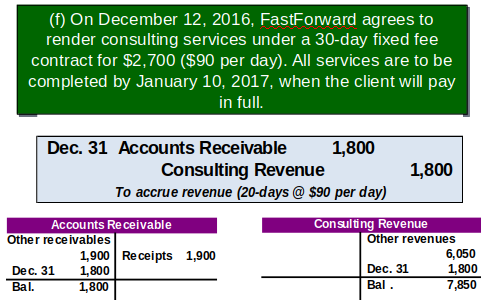
\includegraphics[width=0.9\columnwidth]{images/c3/accrued_revenue_eg1.png}
		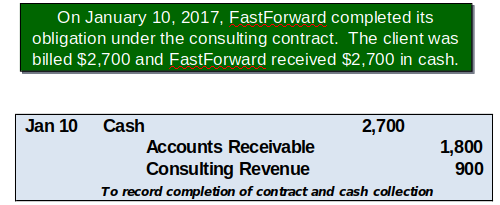
\includegraphics[width=0.9\columnwidth]{images/c3/accrued_revenue_eg2.png}
		\caption{Accrued Revenues Example}	
	\end{figure}
	
	The adjusting entries to record accrued revenue will always debit, or 
	increase, an asset account and credit, or increase, a revenue account.
	
	\subsubsection{Additional Comments}
	
	There are two final points to learn:
	\begin{itemize}[noitemsep]
		\item No adjusting journal entries affected the Cash account. Adjusting 
		journal entries never involve cash.
		\item Adjusting entries always include one balance sheet and one income 
		statement account.
	\end{itemize}

	\subsection{Adjustment Analysis, Recording and Summarizing}
	Adjustments are made at the end of each accounting period immediately prior 
	to preparing an \textbf{adjusted trial balance} and financial statements. 
	An adjusted trial balance is prepared to ensure total debits still equal 
	total credits after having posted the adjusting journal entries to the 
	accounts. If the trial balance is in balance, the financial statements can 
	be prepared.
	
	Adjustments involve determining the necessary adjustments to make to the 
	accounting records. To complete this process, you need to know the balance 
	currently reported in each account, then determine what should be reported 
	as the balance, and finally figure out the adjustment that will take you 
	from the current (unadjusted) balance to the desired (adjusted) balance.
	
	Various adjustments must be made to the accounting records when finalizing 
	and preparing the financial statements. These adjustments help to ensure 
	that all revenues and expenses are reported in the period in which they are 
	earned and incurred. Without these adjustments, the financial statements 
	present an incomplete and misleading picture of the company’s financial 
	performance.
	
\end{document}



